\section{Introduction}

Data centers are responsible for driving large-scale web applications such as web search, storage, advertising, and social network composition ~\cite{chen_understanding_2009, alizadeh_data_2010}. These applications generate diverse traffic patterns with strict throughput and latency requirements. In particular, many distributed web applications rely on a workflow patterns in which requests are broken down and distributed to multiple workers, which perform tasks simultaneously and return responses to an aggregator ~\cite{chen_understanding_2009, alizadeh_data_2010}. As a result, data centers need to support bursts of many-to-one traffic traversing shared bottlenecks without affecting the throughput of long-lived flows needed to update and maintain application data ~\cite{alizadeh_data_2010}.

In order to accommodate the workload generated by these applications while maintaining cost efficiency, modern data centers typically feature high speed links with very low propagation delays connecting nodes via low-cost switches with shallow buffers ~\cite{chen_understanding_2009, hamilton_designing_2007, alizadeh_data_2010}. The majority of communication between nodes is over TCP, which was designed based on the characteristics of wide area networks, where round-trip times (RTTs) are orders of magnitude greater than in data centers ~\cite{chen_understanding_2009}. As a result, while traditional TCP congestion control mechanisms which are usually considered ``good enough'' in the context of the internet, TCP does not perform well when faced with traffic patterns typical of data center networks ~\cite{chen_understanding_2009, phanishayee_measurement_2008}. 

In particular, the traffic patterns common to data center networks suffer a number of impairments due to problems with traditional TCP congestion control mechanisms. This paper discusses a number of approaches to TCP congestion control aimed at improving the performance of TCP in data centers. In particular, Data Center TCP (DCTCP) is discussed in depth, and selected key findings are reproduced using the Mininet network emulator.

\section{Data Center Traffic Patterns}

Distributed applications running in modern data centers are based on the \emph{partition/aggregate} design pattern, in which an application is broken in into hierarchical layers and time-sensitive requests at higher layers are divided and delegated to workers in the lower layers. Many workers perform a small component of a task and return a response to an aggregator, which is combined with responses from other workers and passed back up through the hierarchy. An aggregator combines these responses to get a result which can then be sent back to the user. This model is the basis of many data processing frameworks, cluster storage systems, and targeted advertising applications \cite{chen_understanding_2009, dean_mapreduce:_2004, phanishayee_measurement_2008, alizadeh_data_2010}. These applications require extremely low latencies for short query traffic between workers and aggregators, as well as high throughput for long background flows needed to maintain the freshness of application data and update control state at worker nodes ~\cite{alizadeh_data_2010}. 

\subsection{Performance Impairments}

The current state of TCP congestion control underlies a number of problems that make meeting the demands of distributed applications based on the partition/aggregate pattern difficult to accomplish. 

\subsubsection{Incast}

TCP throughput collapse, or \emph{incast congestion}, arises in many-to-one communication patterns where messages from multiple senders to a single receiver are synchronized and must traverse a shared bottleneck. In incast scenarios, throughput at the receiver collapses as the number of concurrent senders increases and incoming packets overwhelm switch buffers, leading to packet loss and high queuing delays ~\cite{chen_understanding_2009, phanishayee_measurement_2008}. Incast congestion emerges in the partition/aggregate pattern commonly used in distributed applications, as responses from workers to a single aggregator must cross a shared bottleneck and tend to be synchronized ~\cite{alizadeh_data_2010}.

\subsubsection{Buffer Bloat and Underflow}

The ``additive increase, multiplicative decrease'' approach to congestion control in traditional TCP implementations causes long flows to build up buffer queue length until a buffer is overwhelmed and packet loss is detected, at which point the sender-side TCP congestion window is cut, and the sender once again begins to slowly increase the send window. In effect, this approach to congestion control leads to queue buildup, or buffer bloat, which causes long queueing delays even in the absense of packet loss. Conversely, when buffers are small, packet loss is mistakenly interpreted as network congestion, leading to underutilization of network resources \cite{cardwell_bbr:_2016}.

In data centers, this causes latency critical query traffic to incur queuing delays in the presence of long-lived background flows, which steadily build up and maintain large buffer queues. Moreover, improving resource utilization through dynamic buffer allocation means that long lived flows can also cause buffer pressure that impacts flows traversing different ports on the same switch ~\cite{alizadeh_data_2010}.

\section{Improving TCP for Data Centers}

As a result of the performance impairments discussed above, developers have adopted provisional solutions that incur performance costs that impact the overall usefulness of the application. For example, incast congestion can be avoided by adding random delays to query traffic, which reduces the overall response time at higher levels of the hierarchy ~\cite{alizadeh_data_2010, floyd_synchronization_1994}. The solutions presented here attempt to address issues underlying incast congestion and buffer utilization problems by overhauling TCP's congestion control mechanisms and making use of multiple paths available in highly connected data center networks.

\subsection{Data Center TCP}

Data center TCP (DCTCP) attempts to address the problem of latency in partition/aggregate traffic by reducing queue length without affecting throughput for large TCP flows. A DCTCP sender estimates the number of packets marked by the switch based on Explicit Congestion Notification (ECN) feedback from the receiver, and uses this information to reduce its window based on the ratio of marked packets. 

\subsection{Incast Congestion Control for TCP}

Incast Congestion Control for TCP (ICTCP) seeks to improve performance of existing TCP implementations in data center environments by implementing connection throttling mechanisms on the receiver side in an effort to prevent the onset incast congestion. Since incast congestion typically manifests at the last hop switch before synchronized traffic arrives at the receiver, an ICTCP receiver throttles incoming connections on a given interface by measuring the throughput of incoming connections and adjusting the TCP receive window to prevent incoming connections from overwhelming the last hop switch. The TCP receive window is intended as a flow control mechanism designed to prevent a sender from overwhelming the receiver. ICTCP leverages this mechanism as a form of congestion avoidance by setting the receive window for each incoming connection such that their combined throughput will not fill buffers in the last hop switch faster than it can be pushed out onto the link ~\cite{wu_ictcp:_2013}. 

In practice, ICTCP is effective at avoiding incast congestion, but does not fully utilize bandwidth when the number of senders is small ~\cite{wu_ictcp:_2013}. Interestingly, ICTCP outperforms DCTCP in terms of packet loss when many senders send highly synchronized bursts of data ~\cite{wu_ictcp:_2013, alizadeh_data_2010}. Where DCTCP responds to incast congestion after congestion is detected at the switch, ICTCP's uses an ``available bandwidth'' based slow start mechanism and focuses on congestion avoidance, which enables ICTCP receivers to deal with many concurrent, highly synchronized senders without incurring packet loss \cite{alizadeh_data_2010, wu_ictcp:_2013}.

\subsection{Multipath TCP}

\subsection{TCP BBR}

TCP BBR (Bottleneck, Bandwidth, and Round-trip propagation time) uses ``congestion-based congestion control'' in place of traditional loss-based congestion detection mechanisms to improve the performance of TCP. TCP BBR is intended as a general replacement for traditional TCP congestion control mechanisms, though it is currently being implemented in a number of Google services including the Google Cloud Platform as well as Google's B4 Backbone, which is a wide area network comprised of shallow buffered commodity switches similar to those used in data centers ~\cite{cardwell_bbr:_2016, cardwell_tcp_2017}. 

\section{Reproducing Key DCTCP Results}

\subsection{Methods and Results}

Selected results from \cite{alizadeh_data_2010} were reproduced using the Mininet network emulator running on Ubuntu 12.04 with a version of the 3.2.18 Linux kernel patched to add in support for DCTCP. While the original study used link speeds of 1 Gbps and 10 Gbps, initial tests showed Mininet was unable to maintain consistent throughput above 100 Mbps even when running on a compute optimized EC2 instance with support for high bandwidth networking (see Limitations). Thus, a link speed of 100 Mbps was used in all tests in order to acheive consistent results.

\subsubsection{Queue Length}

In order to replicate the queue length results shown in Figures 1 and 13 ~\cite{alizadeh_data_2010}, a simple topology of $N$ flows was constructed with $N$ senders continuously transferring data to a single receiver over a shared bottleneck with a maximum queue length of 400 packets. Figure 1 shows queue length over time for two sustained flows over the shared bottleneck. DCTCP maintained a small steady queue length ($M = 19.38$), while TCP New Reno kept the buffers consistently full with much greater variance in queue length ($M = 330.31$), and exhibited the characteristic sawtooth pattern, with the buffer reaching maximum occupancy at 400 packets before dropping when a loss was detected. Furthermore, Figure 2 shows that DCTCP was much less sensitive to $N$, and maintained consistently low queue sizes at both $N = 2$ and $N = 20$ ($M = 23.63$), whereas queue length for TCP New Reno was consistently greater at $N = 20$ ($M = 368.99$) than when $N = 2$.

\begin{figure}
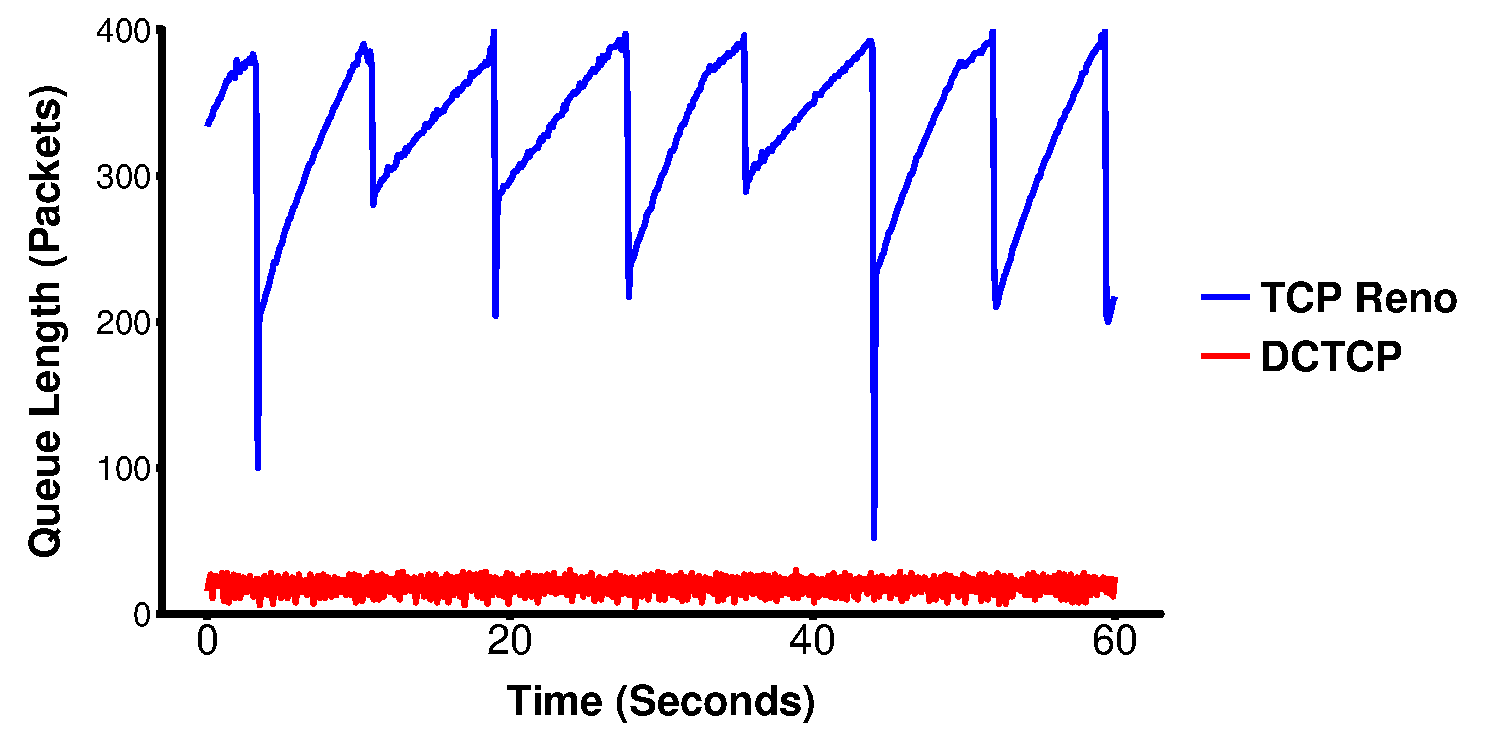
\includegraphics[height=1.75in,width=3.5in]{queue_2_flows}
\caption{Comparison of queue length over time between DCTCP and TCP Reno with 2 flows}
\end{figure}

\begin{figure}
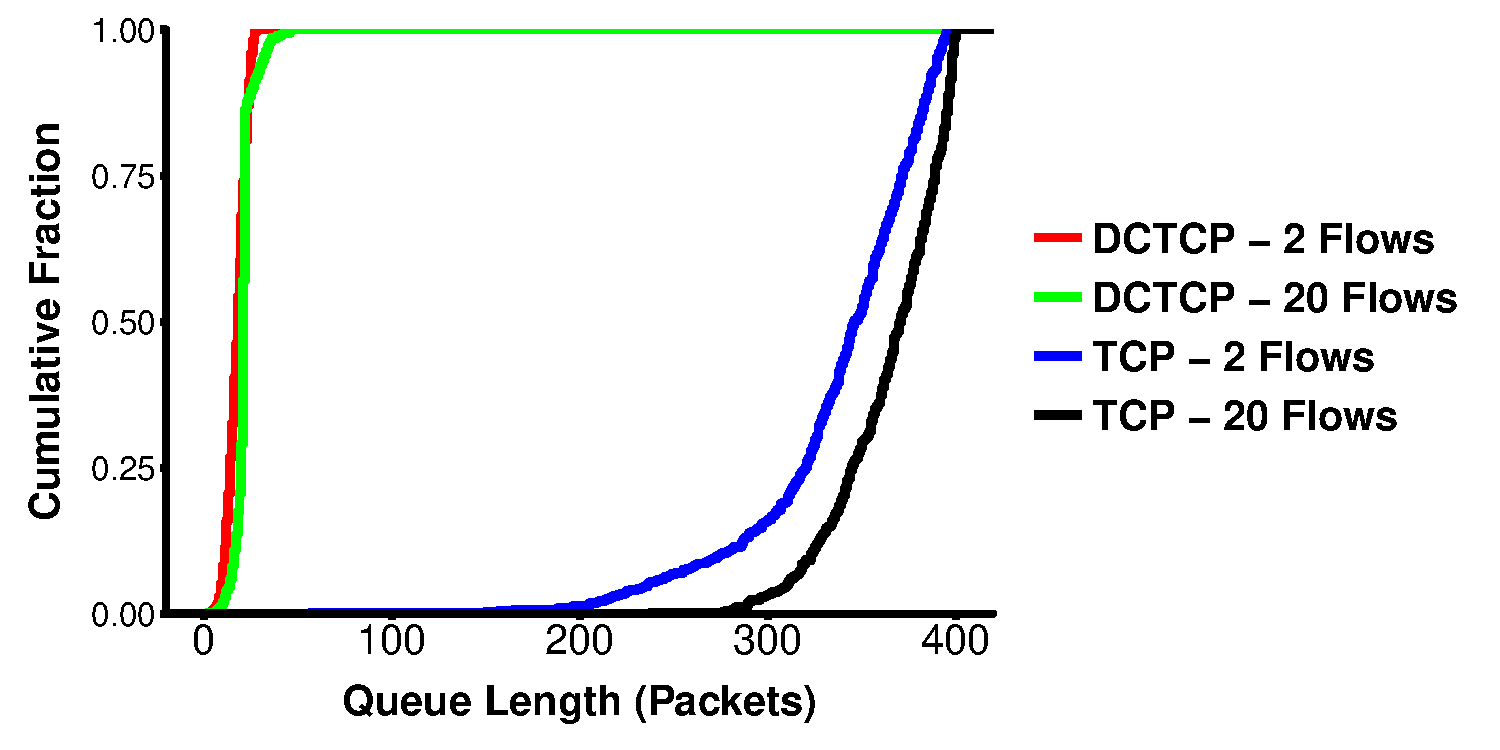
\includegraphics[height=1.75in,width=3.5in]{queue_cdf}
\caption{CDF of queue length for DCTCP and TCP Reno with 2 and 20 flows}
\end{figure}

\subsubsection{Throughput}

 Both DCTCP and TCP New Reno made nearly full use of the 100 Mbps bandwidth, maintaining an average of 98.56 and 98.39 Mbps throughput respectively for $N = 2$, which is consistent with the results of the original paper \cite{alizadeh_data_2010}.

The model presented by the authors suggests setting $K$ as a function of both link speed and RTT, and showed that throughput was insensitive to low values of $K$ at link rates of 1Gbps. Since an initial attempt to reproduce these findings with an RTT of 100$\mu$s at a link speed of 100 Mbps confirmed that throughput was insensitive to $K$, the RTT was increased to 10 ms to compensate for limited bandwidth and the test was repeated. Figure 3 shows the total throughput of two flows transferring data to a single receiver as a function of the marking threshold, $K$. The results under these conditions showed that throughput increased with $K$ until the maximum throughput was reached at $K \approx 12$. 

\begin{figure}
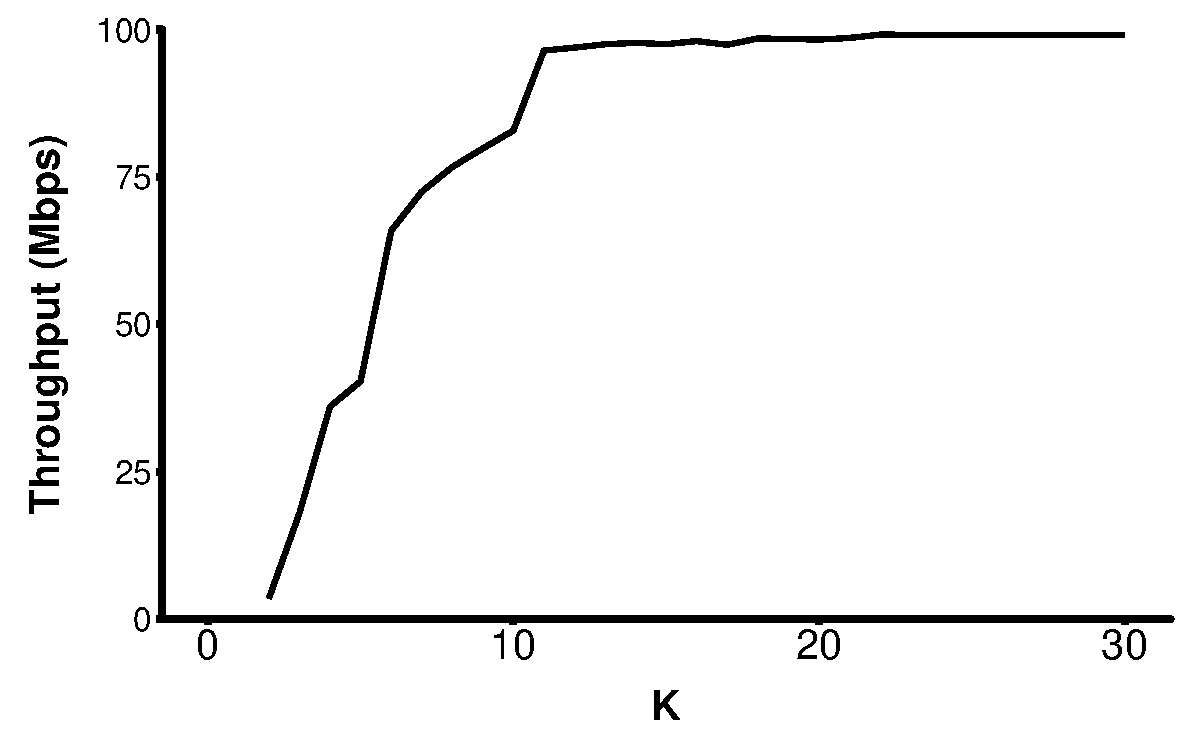
\includegraphics[height=1.75in,width=3in]{k_throughput_delay}
\caption{Throughput as a function of K}
\end{figure}

\subsubsection{Convergence}

Convergence was tested by incrementally starting 5 flows transmitting to a single receiver across a shared bottleneck and allowing each to run for 60 seconds before adding the next flow. Once the fifth flow had run for 60 seconds, each of the 5 flows was stopped in 60 second intervals. The results of the DCTCP convergence test (Figure 4) show that each of the DCTCP flows quickly converges to its fair share of the available bandwidth with little variability. In addition, the total bandwidth across the flows indicated consistently high throughput as flows were started and stopped.

Interestingly, the results of the TCP New Reno convergence test showed considerably more variability.  

\begin{figure}
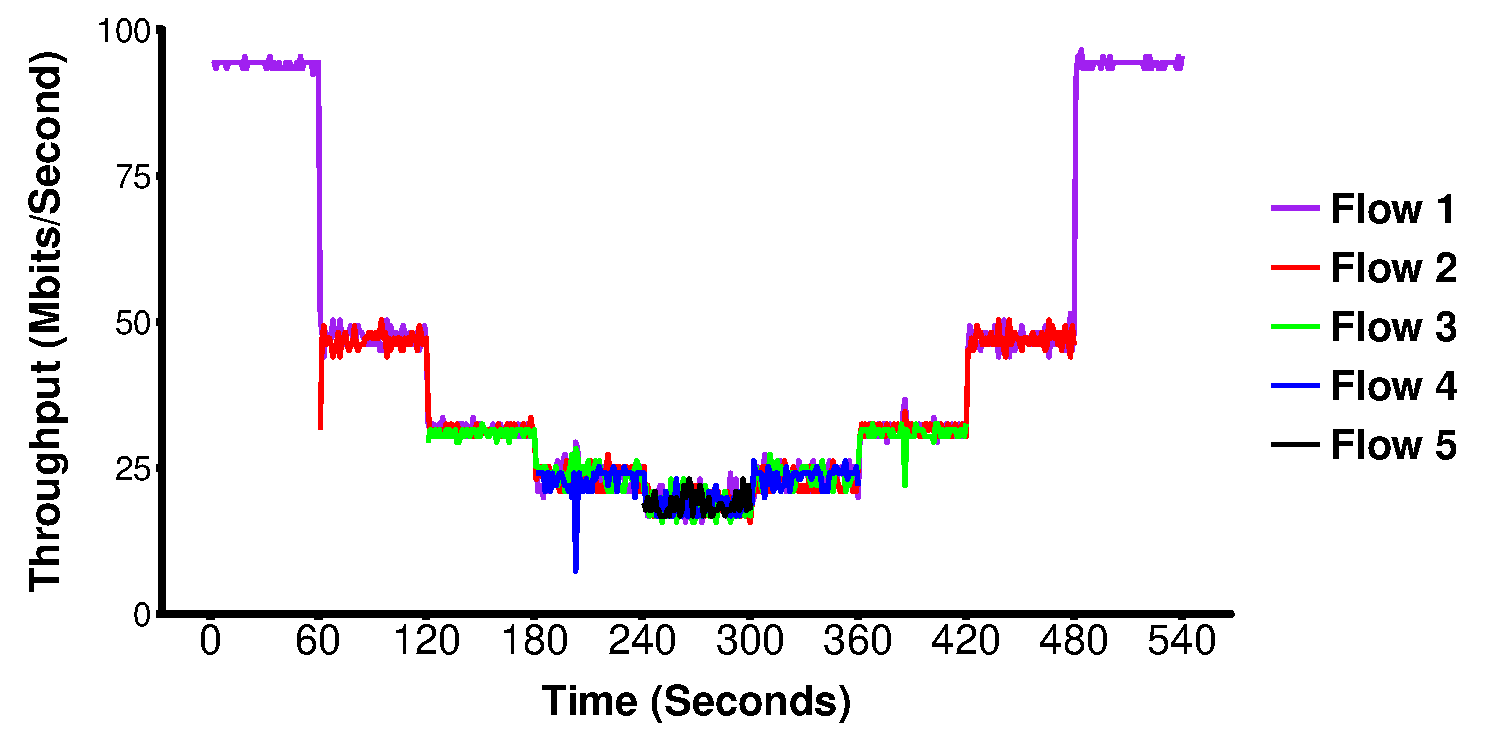
\includegraphics[height=1.75in,width=3.5in]{dctcp_converg}
\caption{Convergence of 5 flows DCTCP}
\end{figure}

\begin{figure}
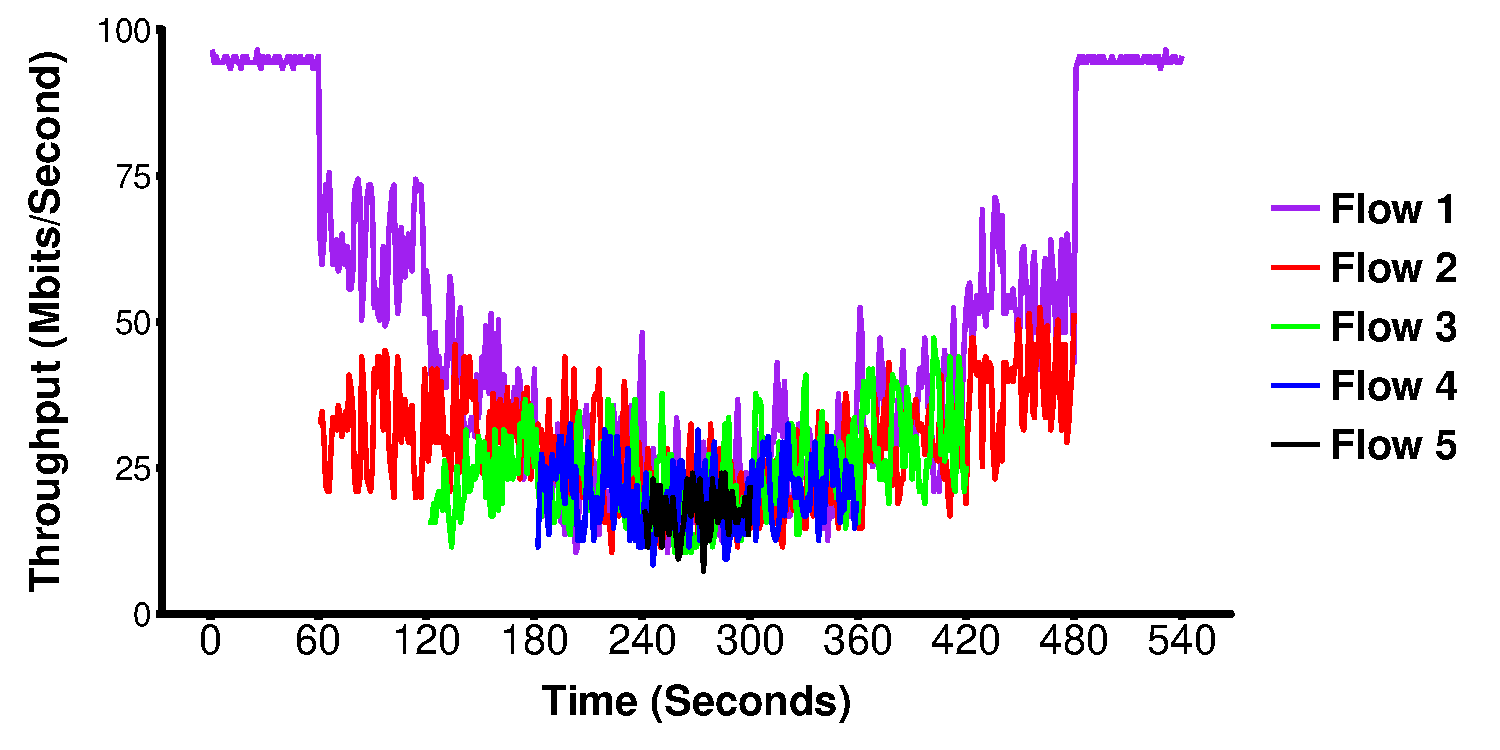
\includegraphics[height=1.75in,width=3.5in]{reno_converg}
\caption{Convergence of 5 flows TCP Reno}
\end{figure}

\subsection{Limitations}

\section{Conclusions}

